\documentclass[aspectratio=169]{beamer}

\usetheme{metropolis}           % Use metropolis theme
\usepackage[utf8]{inputenc}
\usepackage{graphicx}
\usepackage{eso-pic}
\usepackage{graphics}
\usepackage{tikz}
\usepackage[export]{adjustbox}
\usepackage{multicol}
\usepackage{listings}
\usepackage{helvet}
\usepackage{booktabs}
\usepackage{threeparttable}
\usepackage{marvosym}
\usepackage{hyperref}
\usepackage{xcolor}
\usepackage{soul}	% For strike-through
\usepackage{tcolorbox} % For color box

\newcounter{exercises}

\title{Data Processing in Python\\Using Pandas}
\date{}
\author{DIME Analytics \newline Presented by Luis Eduardo San Martin} % Name of author(s) of session here
\institute{Development Impact Evaluation (DIME) \newline The World Bank }
\setbeamercolor{background canvas}{bg=white}	% Sets background color

% The below command places the World Bank logo and DIME logo to the right corner
\titlegraphic{%
	\begin{picture}(0,0)
	\put(330,-180){\makebox(0,0)[rt]{
\includegraphics[width=3cm]{img/WB_logo}}}
	\end{picture}%
	\begin{picture}(0,0)
	\put(390,-180){\makebox(0,0)[rt]{
\includegraphics[width=1.5cm]{img/i2i}}}
	\end{picture}%
}

%%% Section page with picture of Light bulb
\makeatletter
\defbeamertemplate*{section page}{mytheme}[1][]{
	\centering
	\begin{minipage}{22em}
		\raggedright
		\usebeamercolor[fg]{section title}
		\usebeamerfont{section title}
		\par
		\ifx\insertsubsectionhead\@empty\else%
		\usebeamercolor[fg]{subsection title}%
		\usebeamerfont{subsection title}%
		\fi
		\ifstrempty{#1}{}{%
			\includegraphics[width=100mm, height=60mm]{#1}%
		}
		\\
		\insertsectionhead\\[-1ex]
		\insertsubsectionhead
		\usebeamertemplate*{progress bar in section page}
		
	\end{minipage}
	\par
	\vspace{\baselineskip}
}
\makeatother

%%% Define a command to include picture in section, 
%%% make section, and revert to old template
\newcommand{\sectionpic}[2]{
	\setbeamertemplate{section page}[mytheme][#2]
	\section{#1}
	\setbeamertemplate{section page}[mytheme]
}

%%% The command below allows for the text that contains Stata code
\lstset{ %
	backgroundcolor=\color{white},
	basicstyle=\tiny,
	breakatwhitespace=false,
	breaklines=true,
	captionpos=b,
	commentstyle=\color{green},
	escapeinside={\%*}{*)},
	extendedchars=true,
	frame=single,
	numbers=left,
	numbersep=5pt,
	numberstyle=\tiny\color{gray},
	rulecolor=\color{black},
	showspaces=false,
	showstringspaces=false,
	showtabs=false,
	stringstyle=\color{mauve},
	tabsize=2,
	title=\lstname,
	morekeywords={not,\},\{,preconditions,effects },
	deletekeywords={time}
}

%% The below command creates the ligh bulb logos in the top right corner of the 
\begin{document}
	
	
	%%%%%%%%%%%%%%%%%%%%%%%%%%%%%%%%%%%%%%%%%%% Title slide
	{
		\usebackgroundtemplate{
\includegraphics[height=55mm,right]{img/top_right_corner.pdf}} 
		\maketitle
	}

\begin{frame}

	\frametitle{Overview} % Table of contents slide, comment this block out to remove it
	\tableofcontents % Throughout your presentation, if you choose to use \section{} and \subsection{} commands, these will automatically be printed on this slide as an overview of your presentation

\end{frame}

%%%%%%%%%%%%%%%%%%%%%%%%%%%%%%%%%%%%%%%%%%% Section title slide
\sectionpic{Introduction}{img/section_slide}

%%%%%%%%%%%%%%%%%%%%%%%%%%%%%%%%%%%%%%%%%%% Slide
\begin{frame}{Introduction}

	\begin{itemize}
		\item This session will introduce you to Pandas
		\item Pandas are the most popular way to store and process data in Python
		\item We'll discuss:
		\begin{itemize}
			\item Pandas dataframes
			\item Data processing operations
		\end{itemize}
		\item We'll compare Pandas' commands to commands in Stata
	\end{itemize}

\end{frame}

%%%%%%%%%%%%%%%%%%%%%%%%%%%%%%%%%%%%%%%%%%% Slide
\begin{frame}{Introduction}

	\textbf{Why Pandas if I already know Stata?}

	\begin{itemize}
		\item \textbf{General Python data work:} Almost all Python data work libraries builds on Pandas
		\item \textbf{ML:} If you ever want to implement machine learning using Python, you'll likely need Pandas
		\item \textbf{Cloud platforms:} Cloud platforms assume Python much more often than Stata, and Pandas is the library assumed for data processing
		\item \textbf{Big data:} though Pandas is not suitable for big data,  the most popular Python big data tools expect you to know it
		
	\end{itemize}

\end{frame}

%%%%%%%%%%%%%%%%%%%%%%%%%%%%%%%%%%%%%%%%%%% Slide
\begin{frame}{Introduction}

	\textbf{Getting started}

	\begin{itemize}
		\item We'll use \href{http://colab.research.google.com}{Google Colab} today
		\item It is similar to a Google Doc but for coding, and runs Python by default
	\end{itemize}

\end{frame}

%%%%%%%%%%%%%%%%%%%%%%%%%%%%%%%%%%%%%%%%%%% Slide
\begin{frame}{Introduction}

	\textbf{Getting started}

	\begin{itemize}
		\item Go to https://colab.research.google.com
		\item Click on \texttt{NEW NOTEBOOK} if you're already logged in, or go to \texttt{File > New notebook} if you're not
	\end{itemize}

	\begin{multicols}{2}

		\begin{figure}
			\centering
			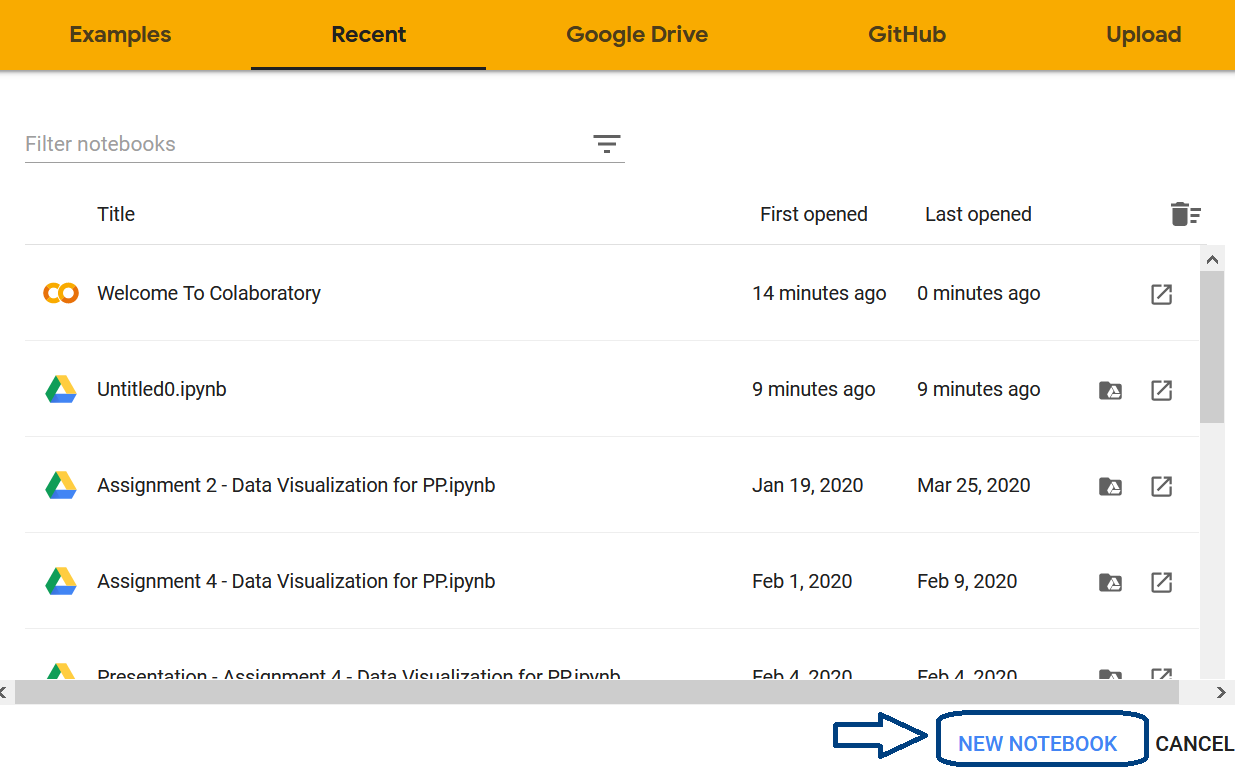
\includegraphics[width=0.85\linewidth]{img/new_nb_logged_in.png}
			\caption{Do this if you're already logged in}
		\end{figure}
		\begin{figure}
			\centering
			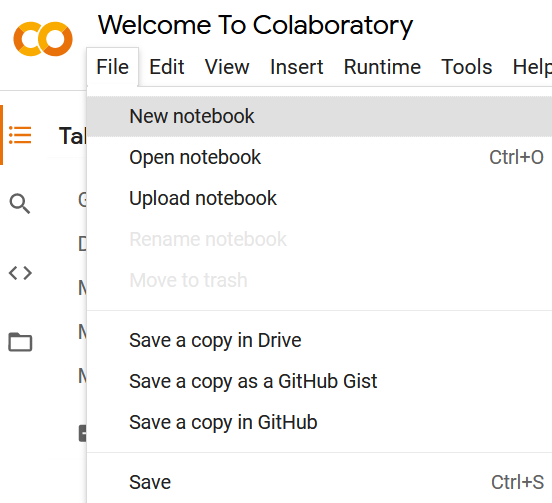
\includegraphics[width=0.55\linewidth]{img/new_nb_not_logged_in.png}
			\caption{Do this if you're not -- you'll be prompted to log in}
		\end{figure}

	\end{multicols}

\end{frame}

%%%%%%%%%%%%%%%%%%%%%%%%%%%%%%%%%%%%%%%%%%% Section title slide
\sectionpic{Pandas}{img/section_slide}

%%%%%%%%%%%%%%%%%%%%%%%%%%%%%%%%%%%%%%%%%%% Slide
\begin{frame}{Pandas}

	\textbf{The Pandas library}

	\begin{itemize}
		\item Pandas is an external library for Python, it isn't part of Python's base installation
		\item In Google colab it is already installed, but you will have to install it using \texttt{pip install pandas}
		\item Use the following command to import Pandas to your notebook:
	\end{itemize}

	\hspace{7mm} \texttt{\textcolor{purple}{import} pandas as \textcolor{purple}{pd}}

\end{frame}


%%%%%%%%%%%%%%%%%%%%%%%%%%%%%%%%%%%%%%%%%%% Slide
\begin{frame}{Pandas}

	\textbf{Dataframes}

	\begin{multicols}{2}
	
		\begin{itemize}
			\item A dataframe is a two-dimensional data structure
			\item The Stata equivalent to dataframes are datasets
			\item Dataframes is a data structure where each row represents a unit of observation and each column represents an observation's attribute		
		\end{itemize}
		\begin{figure}
			\centering
			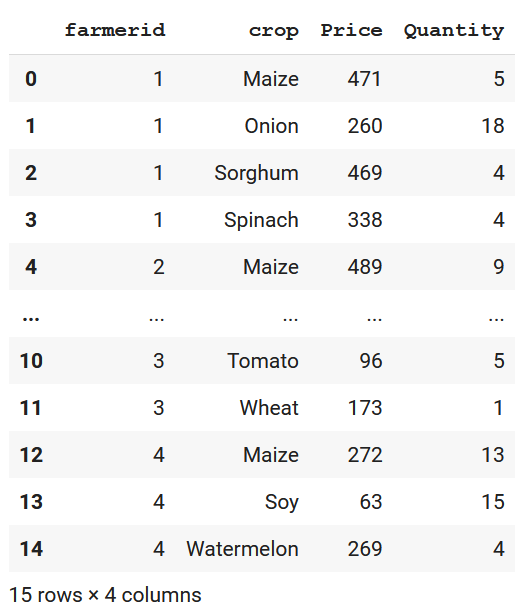
\includegraphics[width=0.8\linewidth]{img/dataframe.png}
		\end{figure}

	\end{multicols}

\end{frame}

%%%%%%%%%%%%%%%%%%%%%%%%%%%%%%%%%%%%%%%%%%% Slide
\begin{frame}{Pandas}

	\textbf{Creating a dataframe}

	There are several ways to create a dataframe from scratch. One of the easiest is:

	\begin{enumerate}
		\item Define a list of strings with the column names
		\begin{figure}
			
\includegraphics[width=0.8\linewidth]{img/column_names.png}
		\end{figure}
		\item Define a list for \textbf{each observation}
		\begin{figure}
			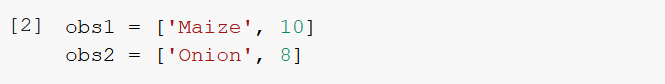
\includegraphics[width=0.8\linewidth]{img/observation_lists.png}
		\end{figure}
		\item Wrap all of the observation lists in another list
		\begin{figure}
			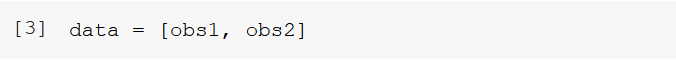
\includegraphics[width=0.8\linewidth]{img/data_list.png}
		\end{figure}

	\end{enumerate}

\end{frame}

%%%%%%%%%%%%%%%%%%%%%%%%%%%%%%%%%%%%%%%%%%% Slide
\begin{frame}{Pandas}

	\textbf{Creating a dataframe}

	\begin{enumerate}
		\setcounter{enumi}{3}
		\item Use the lists \texttt{data} and \texttt{column\_names} as inputs in the \texttt{DataFrame()} command
		\begin{figure}
			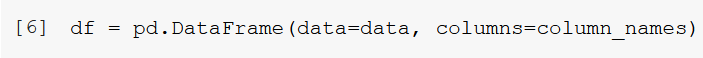
\includegraphics[width=0.8\linewidth]{img/dataframe_definition.png}
		\end{figure}
		\item Now your dataframe is defined in the variable \texttt{df}. You can use that name to refer to it or print it, as in:
		\begin{figure}
			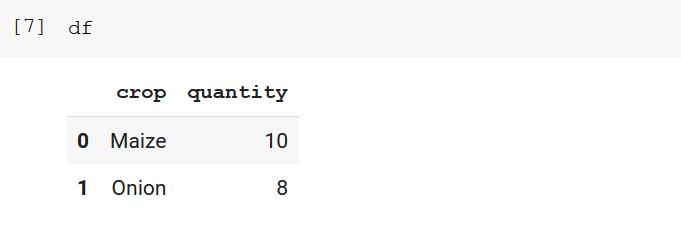
\includegraphics[width=0.8\linewidth]{img/df.png}
		\end{figure}
	\end{enumerate}

\end{frame}

%%%%%%%%%%%%%%%%%%%%%%%%%%%%%%%%%%%%%%%%%%% Slide
\begin{frame}{Pandas}

	\textbf{Creating a dataframe}

	Another way to create a dataframe from zero is to define an empty dataframe and then create its columns individually.
	\begin{figure}
		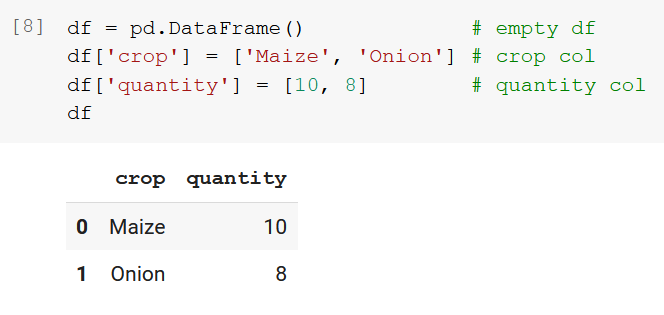
\includegraphics[width=0.8\linewidth]{img/df_definition2.png}
	\end{figure}

\end{frame}



%%%%%%%%%%%%%%%%%%%%%%%%%%%%%%%%%%%%%%%%%%% Section title slide
\sectionpic{Importing and exploring data}{img/section_slide}


%%%%%%%%%%%%%%%%%%%%%%%%%%%%%%%%%%%%%%%%%%% Slide
\begin{frame}{Reading and exploring data}

	\textbf{Importing data to a dataframe from a file}

	\begin{itemize}
		\item In our work, we don't usually need to define a dataframe from scratch
		\item More often, we load pre-existing data files
		\item To load a \texttt{.csv} file into a dataframe, we use the command \texttt{read\_csv()}
	\end{itemize}

\end{frame}

%%%%%%%%%%%%%%%%%%%%%%%%%%%%%%%%%%%%%%%%%%% Slide
\begin{frame}{Reading and exploring data}

	\textbf{Importing data to a dataframe from a file}

	\texttt{pd.read\_csv()}

	\begin{figure}
		\centering
		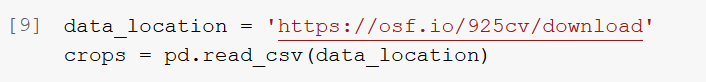
\includegraphics[width=0.9\linewidth]{img/read_csv.png}
	\end{figure}

\end{frame}

%%%%%%%%%%%%%%%%%%%%%%%%%%%%%%%%%%%%%%%%%%% Slide
\begin{frame}{Reading and exploring data}

	\textbf{Importing data to a dataframe from a file}

	\texttt{pd.read\_csv()}

	\begin{figure}
		\centering
		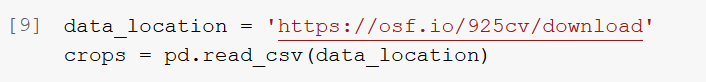
\includegraphics[width=0.9\linewidth]{img/read_csv.png}
	\end{figure}
	\begin{itemize}
		\item \texttt{data\_location} is a string with the location of our file
		\item It can be a URL or a path in your local disk -- though a path in your local disk won't work directly with Colab
		\item \texttt{read\_csv()} is the Pandas function to read \texttt{.csv} files into dataframes. It takes the file location string as input
	\end{itemize}

\end{frame}

%%%%%%%%%%%%%%%%%%%%%%%%%%%%%%%%%%%%%%%%%%% Slide
\begin{frame}{Reading and exploring data}

	\textbf{Importing data to a dataframe from a file}

	\begin{figure}
		\centering
		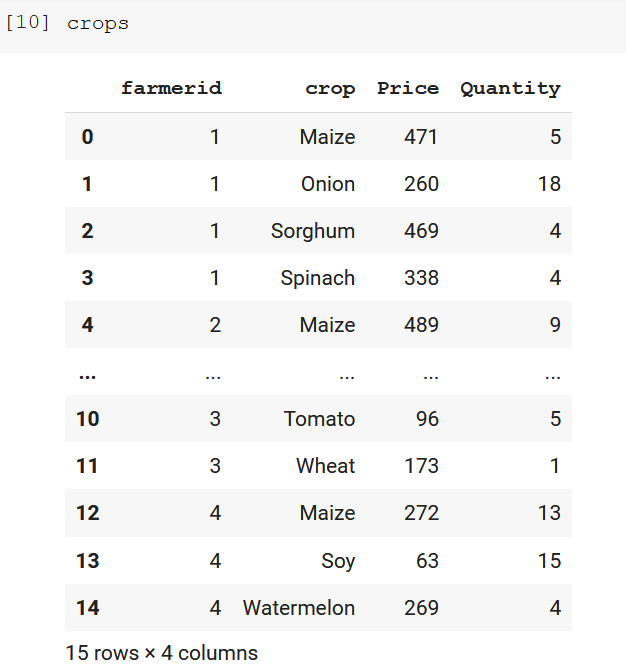
\includegraphics[width=0.4\linewidth]{img/crops_df.png}
	\end{figure}

\end{frame}

%%%%%%%%%%%%%%%%%%%%%%%%%%%%%%%%%%%%%%%%%%% Slide
\begin{frame}{Reading and exploring data}

	\textbf{Exploring a dataframe}

	\begin{multicols}{2}

		Running the dataframe name as a command will print it. If the dataframe has too many rows or columns, Python will print only the first and last rows and columns.

		\begin{figure}
			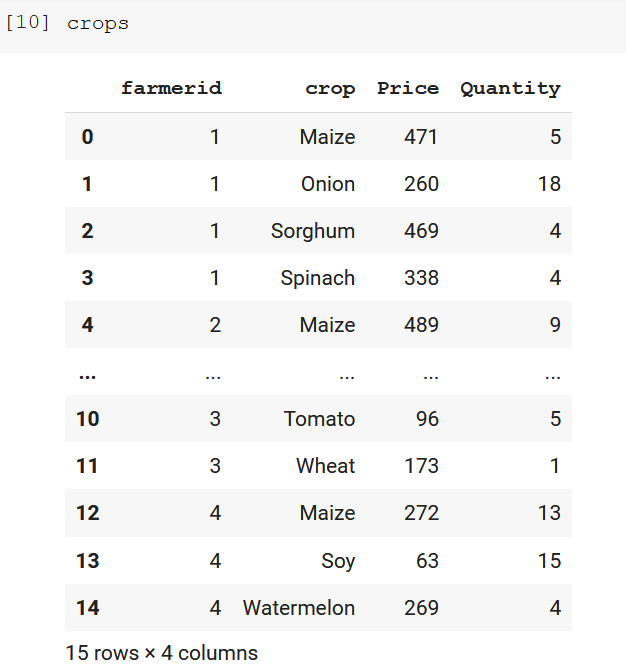
\includegraphics[width=0.85\linewidth]{img/crops_df.png}
		\end{figure}

	\end{multicols}{2}

\end{frame}

%%%%%%%%%%%%%%%%%%%%%%%%%%%%%%%%%%%%%%%%%%% Slide
\begin{frame}{Reading and exploring data}

	\textbf{Exploring a dataframe}

	We can also use the \texttt{.head()} and \texttt{.tail()} attributes to return the first and last observations of a dataframe

	\begin{multicols}{2}

		\begin{figure}
			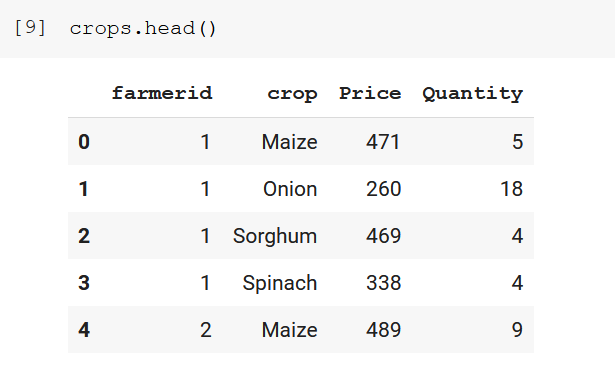
\includegraphics[width=\linewidth]{img/head.png}
		\end{figure}
		\begin{figure}
			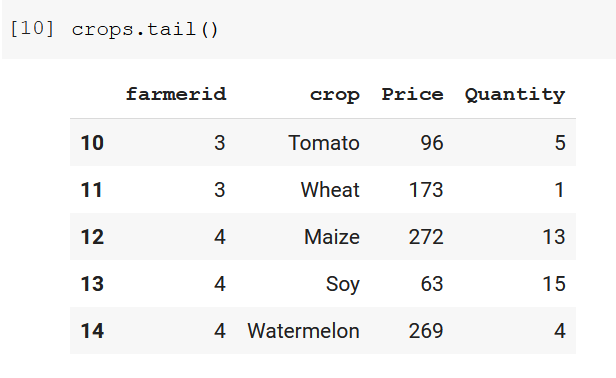
\includegraphics[width=\linewidth]{img/tail.png}
		\end{figure}

	\end{multicols}

\end{frame}

%%%%%%%%%%%%%%%%%%%%%%%%%%%%%%%%%%%%%%%%%%% Slide
\begin{frame}{Reading and exploring data}

	\textbf{Exploring a dataframe}

	To see how many rows and columns a dataframe has, we use the \texttt{.shape} attribute:
	
	\begin{figure}
		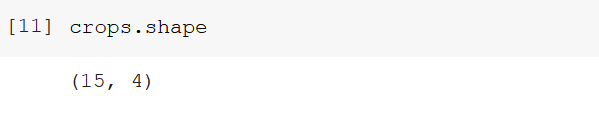
\includegraphics[width=0.7\linewidth]{img/crops_shape.png}
	\end{figure}

	The result is a tuple (an immutable list) whose elements are the number of rows and columns

\end{frame}

%%%%%%%%%%%%%%%%%%%%%%%%%%%%%%%%%%%%%%%%%%% Slide
\begin{frame}{Reading and exploring data}

	\textbf{Exploring a dataframe}

	We can also get the number of rows with the \texttt{len()} function:
	
	\begin{figure}
		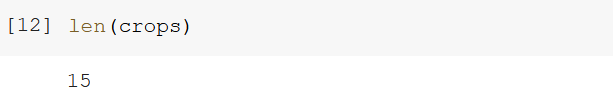
\includegraphics[width=0.7\linewidth]{img/crops_len.png}
	\end{figure}
	
	The result of \texttt{len()} is an integer.

\end{frame}

%%%%%%%%%%%%%%%%%%%%%%%%%%%%%%%%%%%%%%%%%%% Slide
\begin{frame}{Reading and exploring data}

	\textbf{Exploring a dataframe}

	To check the column names, we use the \texttt{.columns} attribute:
	
	\begin{figure}
		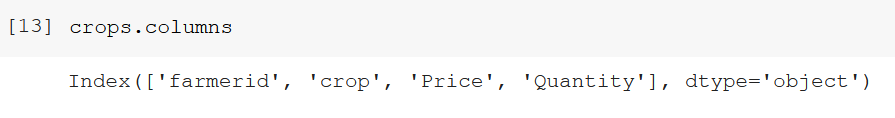
\includegraphics[width=0.9\linewidth]{img/crops_columns.png}
	\end{figure}

\end{frame}

%%%%%%%%%%%%%%%%%%%%%%%%%%%%%%%%%%%%%%%%%%% Section title slide
\sectionpic{Indexing and filtering}{img/section_slide}

%%%%%%%%%%%%%%%%%%%%%%%%%%%%%%%%%%%%%%%%%%% Slide
\begin{frame}{Indexing and filtering}

	\textbf{Dataframe indexing}

	\begin{multicols}{2}

		\begin{itemize}
			\item Every row and column of a dataframe has a \textbf{label}
			\item Row labels are represented by the index
			\item Column labels are represented by the column names
		\end{itemize}
		\begin{figure}
			\centering
			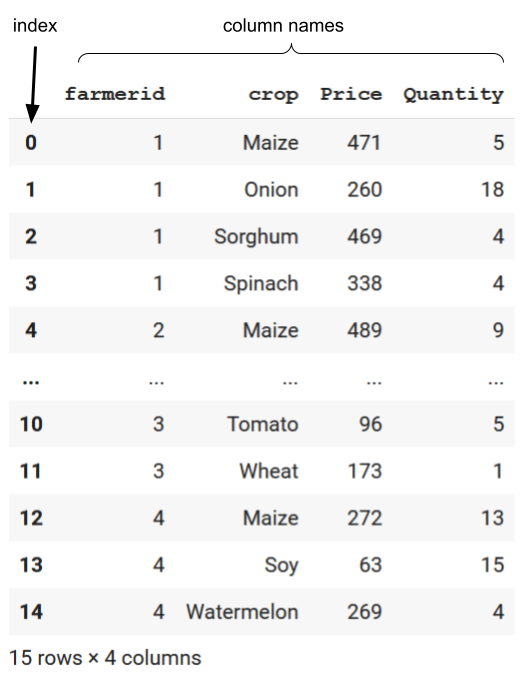
\includegraphics[width=0.71\linewidth]{img/dataframe_indices.png}
		\end{figure}

	\end{multicols}

\end{frame}

%%%%%%%%%%%%%%%%%%%%%%%%%%%%%%%%%%%%%%%%%%% Slide
\begin{frame}{Indexing and filtering}

	\textbf{Column indexing}

	We can subset a single column of a dataframe using two methods:

	\begin{itemize}
		\item \texttt{df.column\_name}
		\item \texttt{df['column\_name']}
	\end{itemize}

\end{frame}

%%%%%%%%%%%%%%%%%%%%%%%%%%%%%%%%%%%%%%%%%%% Slide
\begin{frame}{Indexing and filtering}

	\textbf{Column indexing}

	\begin{multicols}{2}

		\begin{figure}
			\centering
			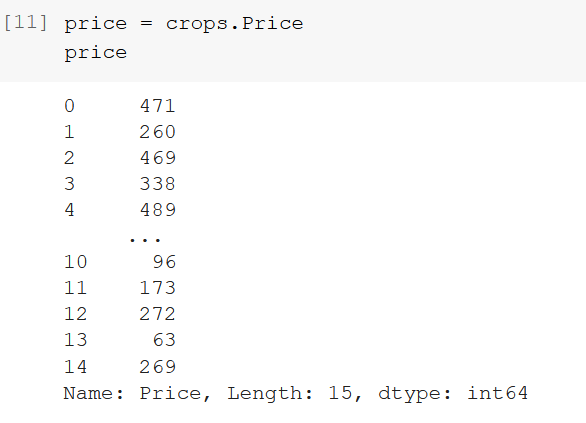
\includegraphics[width=0.95\linewidth]{img/col_subset1.png}
		\end{figure}
		\begin{figure}
			\centering
			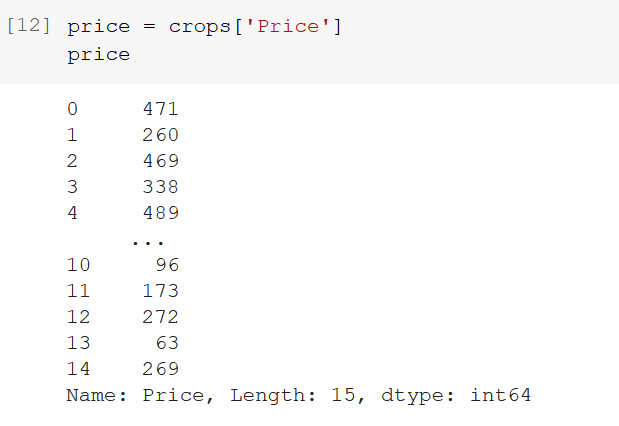
\includegraphics[width=0.99\linewidth]{img/col_subset2.png}
		\end{figure}

	\end{multicols}

\end{frame}

%%%%%%%%%%%%%%%%%%%%%%%%%%%%%%%%%%%%%%%%%%% Slide
\begin{frame}{Indexing and filtering}

	\textbf{Column indexing}

	The difference between the two is that the first method doesn't allow column name references, while the second does
	\begin{figure}
		\centering
		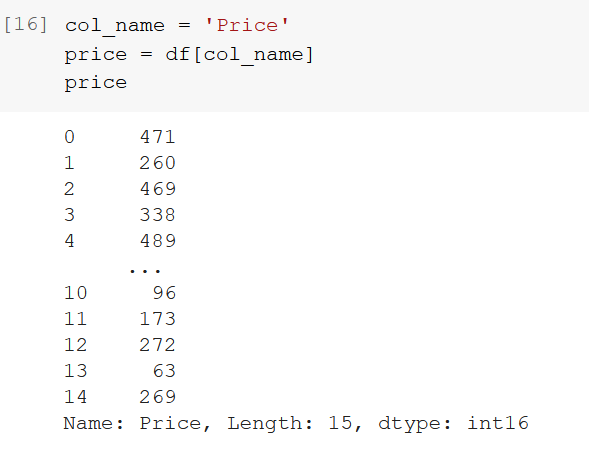
\includegraphics[width=0.47\linewidth]{img/col_name_reference.png}
	\end{figure}

\end{frame}

%%%%%%%%%%%%%%%%%%%%%%%%%%%%%%%%%%%%%%%%%%% Slide
\begin{frame}{Indexing and filtering}

	\textbf{Multi-column indexing}

	\begin{itemize}
		\item We can use a syntax similar to the second method to index more than one column at the same time
		\item Instead of including a string with one column name inside the brackets, we include a list of strings with the column names to index
	\end{itemize}

	\hspace{7mm} \texttt{df[['col\_name1', 'col\_name2', 'col\_name3', ...]]}

	\begin{itemize}
		\item Note that inside the outer brackets we have a list of strings
	\end{itemize}

\end{frame}

%%%%%%%%%%%%%%%%%%%%%%%%%%%%%%%%%%%%%%%%%%% Slide
\begin{frame}{Indexing and filtering}

	\textbf{Multi-column indexing}

	\begin{multicols}{2}

		\begin{figure}
			\centering
			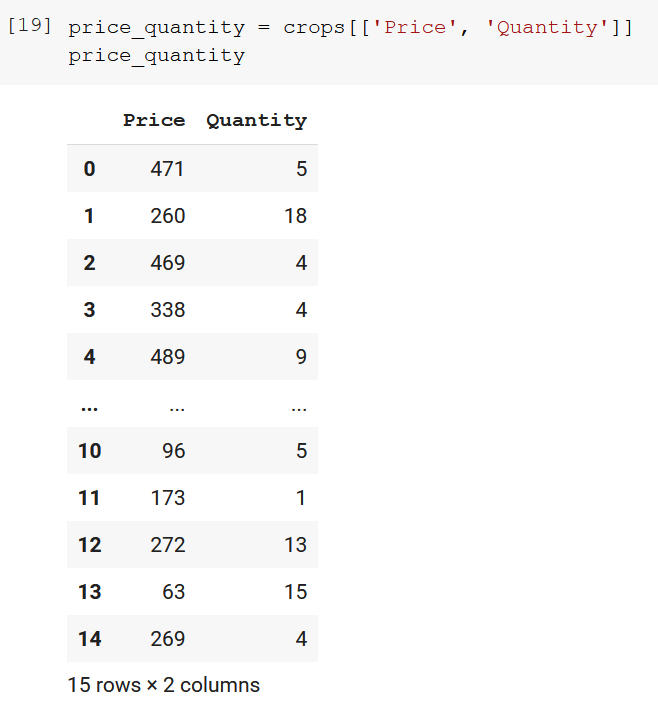
\includegraphics[width=0.8\linewidth]{img/multicol_subsetting1.png}
		\end{figure}
		\begin{figure}
			\centering
			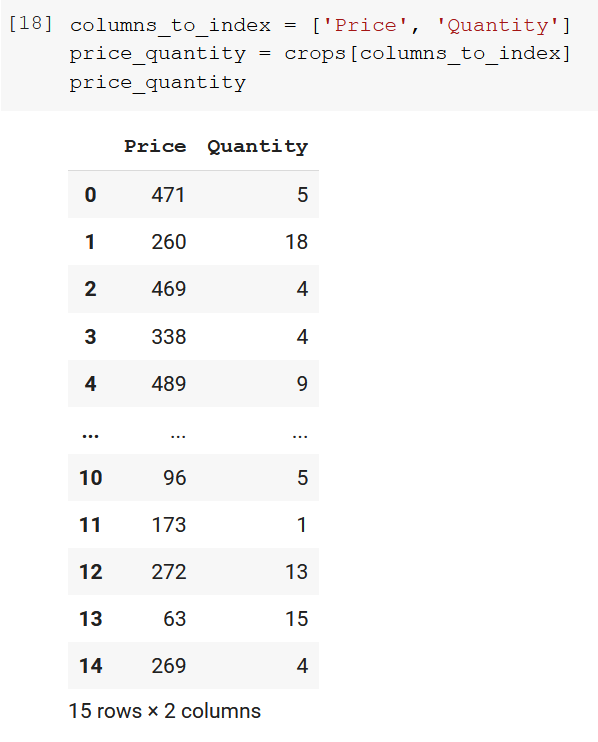
\includegraphics[width=0.75\linewidth]{img/multicol_subsetting2.png}
		\end{figure}

	\end{multicols}

\end{frame}

%%%%%%%%%%%%%%%%%%%%%%%%%%%%%%%%%%%%%%%%%%% Slide
\begin{frame}{Indexing and filtering}

	\textbf{Multi-column indexing}

	A one-column index operation returns a Pandas series. A multicolumn index returns another dataframe.

	\begin{multicols}{2}

		\begin{figure}
			\centering
			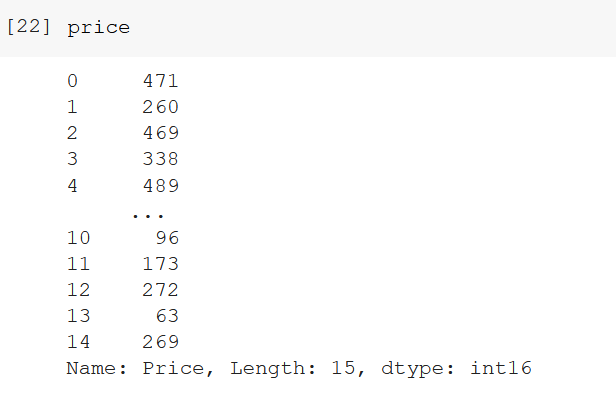
\includegraphics[width=0.7\linewidth]{img/price.png}
		\end{figure}
		\begin{figure}
			\centering
			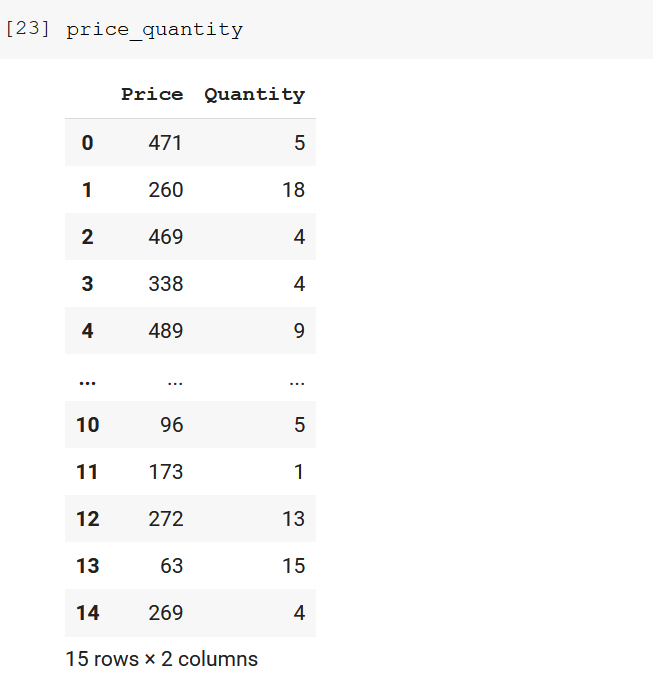
\includegraphics[width=0.7\linewidth]{img/price_quantity.png}
		\end{figure}

	\end{multicols}

\end{frame}

%%%%%%%%%%%%%%%%%%%%%%%%%%%%%%%%%%%%%%%%%%% Slide
\begin{frame}{Indexing and filtering}

	\textbf{Row indexing}

	There are basically two methods to index rows in Pandas. The simplest is \texttt{.iloc[]}, which is used to index the i-th row or rows:

	\begin{itemize}
		\item Indexing a single row: \texttt{df.iloc[i]}
		\item Indexing a range of continuous rows from i until (j-1): \texttt{df.iloc[i:j]}
		\item Indexing the i-th and j-th non-continuous rows: \texttt{df.iloc[[i, j]]}
	\end{itemize}

	\textbf{Very important:} In Python, every numeric index starts at zero, not at one

\end{frame}

%%%%%%%%%%%%%%%%%%%%%%%%%%%%%%%%%%%%%%%%%%% Slide
\begin{frame}{Indexing and filtering}

	\textbf{Row indexing}

	\begin{itemize}
		\item Indexing a single row: \texttt{df.iloc[i]}
	\end{itemize}

	\begin{figure}
		\centering
		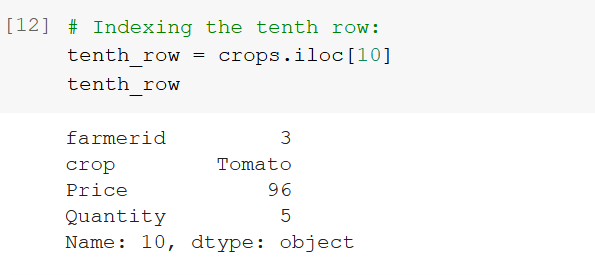
\includegraphics[width=0.6\linewidth]{img/single_row.png}
	\end{figure}

	Note that the outcome of indexing a single row is a Pandas series, not a dataframe

\end{frame}

%%%%%%%%%%%%%%%%%%%%%%%%%%%%%%%%%%%%%%%%%%% Slide
\begin{frame}{Indexing and filtering}

	\textbf{Row indexing}

	\begin{itemize}
		\item Indexing a range of continuous rows from i until (j-1): \texttt{df.iloc[i:j]}
	\end{itemize}

	\begin{figure}
		\centering
		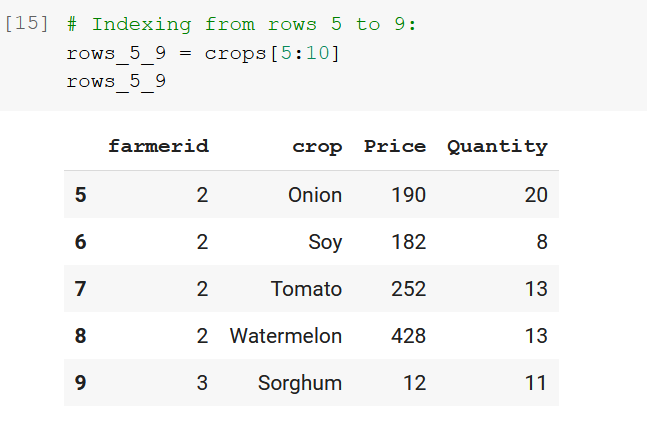
\includegraphics[width=0.5\linewidth]{img/consecutive_rows.png}
	\end{figure}

\end{frame}

%%%%%%%%%%%%%%%%%%%%%%%%%%%%%%%%%%%%%%%%%%% Slide
\begin{frame}{Indexing and filtering}

	\textbf{Row indexing}

	\begin{itemize}
		\item Indexing the i-th and j-th non-continuous rows: \texttt{df.iloc[[i, j]]}
	\end{itemize}

	\begin{figure}
		\centering
		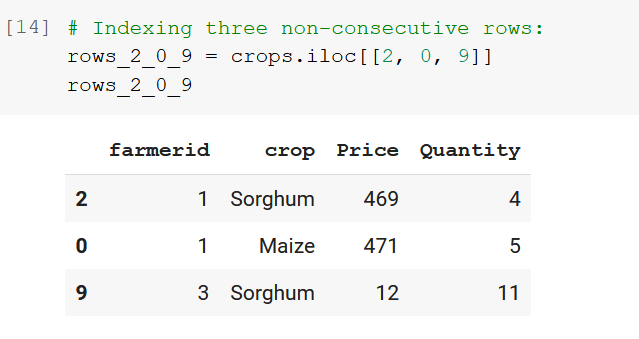
\includegraphics[width=0.5\linewidth]{img/non-consecutive_rows.png}
	\end{figure}

	Note that the index of the resulting dataframe is not necessarily sorted, it keeps the order in which we selected the rows to subset

\end{frame}

%%%%%%%%%%%%%%%%%%%%%%%%%%%%%%%%%%%%%%%%%%% Slide
\begin{frame}{Indexing and filtering}

	\textbf{Row indexing}

	The second method to index rows in Pandas is \texttt{.loc[]}. It subsets the rows whose index values coincide with the input inside the brackets.

	\begin{itemize}
		\item Until now, the dataframes we've worked with had an index which coincided with the row number
		\item That's not always the case, as we'll soon see
		\item The command to index the row whose index value is \texttt{i} is this: \texttt{df.loc[i]}
	\end{itemize}

We'll show more on the diference between the \texttt{.loc[]} and \texttt{iloc[]} methods in the next slide

\end{frame}

%%%%%%%%%%%%%%%%%%%%%%%%%%%%%%%%%%%%%%%%%%% Slide
\begin{frame}{Indexing and filtering}

	\textbf{Row indexing}

	\begin{figure}
		\centering
		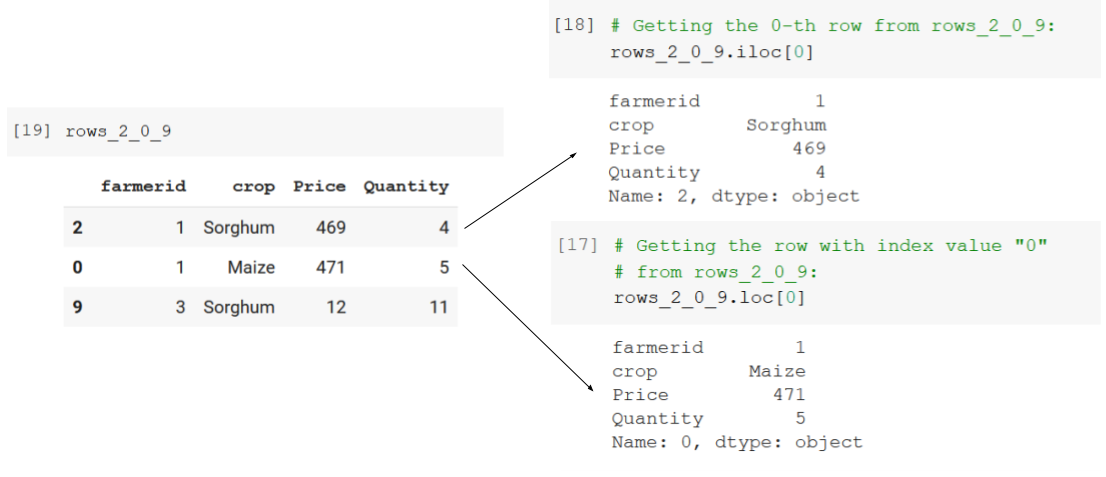
\includegraphics[width=\linewidth]{img/row_loc_iloc.png}
	\end{figure}

\end{frame}

%%%%%%%%%%%%%%%%%%%%%%%%%%%%%%%%%%%%%%%%%%% Slide
\begin{frame}{Indexing and filtering}

	\textbf{Single-value indexing}

	To index a single value of a dataframe, we need to index a column and the row-index value \texttt{.loc[]} or position \texttt{.iloc[]}

	\begin{multicols}{2}

		\begin{figure}
			\centering
			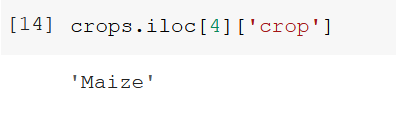
\includegraphics[width=\linewidth]{img/single_value_index1.png}
		\end{figure}
		\begin{figure}
			\centering
			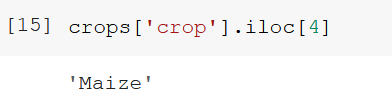
\includegraphics[width=\linewidth]{img/single_value_index2.png}
		\end{figure}

	\end{multicols}

	We can specify the row first and the column later, or viceversa

\end{frame}

%%%%%%%%%%%%%%%%%%%%%%%%%%%%%%%%%%%%%%%%%%% Slide
\begin{frame}{Indexing and filtering}

	\textbf{Filtering}

	\begin{itemize}
		\item In Stata, we use the command \texttt{keep if \textit{column\_condition}} to filter observations
		\item Pandas' syntax to filter is heavier, as we shall see soon
	\end{itemize}

\end{frame}

%%%%%%%%%%%%%%%%%%%%%%%%%%%%%%%%%%%%%%%%%%% Slide
\begin{frame}{Indexing and filtering}

	\textbf{Filtering}

	\begin{itemize}
		\item To filter values of a dataframe, we use brackets and include a list or Pandas series with boolean values inside them:
	\end{itemize}

	\hspace{7mm} \texttt{df[list\_with\_booleans]}

	\begin{itemize}	
		\item The observations filtered-in are the ones that have a value of \texttt{True} in their cooresponding position
	\end{itemize}

\end{frame}

%%%%%%%%%%%%%%%%%%%%%%%%%%%%%%%%%%%%%%%%%%% Slide
\begin{frame}{Indexing and filtering}

	\textbf{Filtering}

	Note that the list or Pandas series with booleans needs to have the same length as the dataframe

	\begin{multicols}{2}

		\begin{figure}
			\centering
			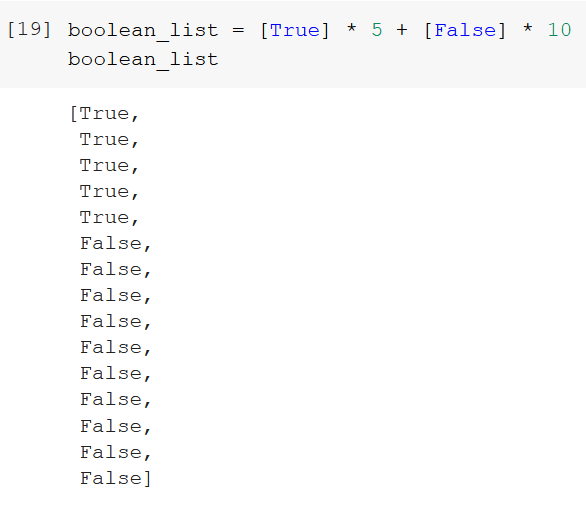
\includegraphics[width=0.85\linewidth]{img/boolean_list.png}
		\end{figure}
		\begin{figure}
			\centering
			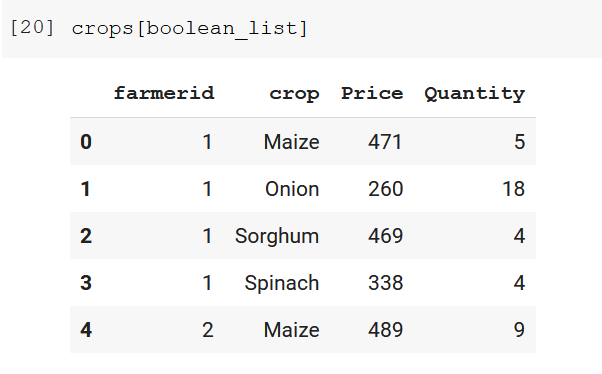
\includegraphics[width=\linewidth]{img/crops_filtered.png}
		\end{figure}

	\end{multicols}

\end{frame}

%%%%%%%%%%%%%%%%%%%%%%%%%%%%%%%%%%%%%%%%%%% Slide
\begin{frame}{Indexing and filtering}

	\textbf{Filtering}

	\begin{itemize}
		\item Other than a list with booleans, we can use a Pandas series with booleans
		\item The advantage of this is that we can generate them very easily when operating a dataframe column with a logical condition
	\end{itemize}

	\begin{figure}
		\centering
		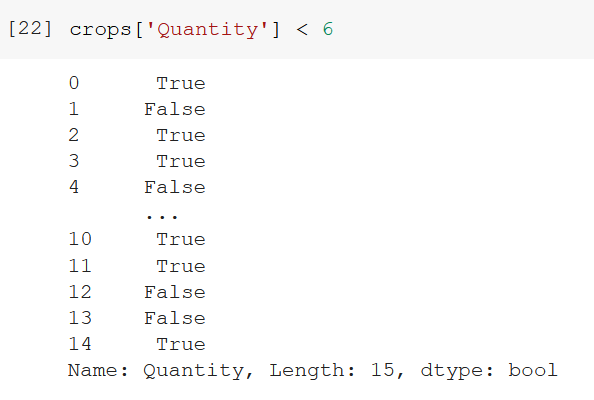
\includegraphics[width=0.45\linewidth]{img/boolean_series.png}
	\end{figure}


\end{frame}

%%%%%%%%%%%%%%%%%%%%%%%%%%%%%%%%%%%%%%%%%%% Slide
\begin{frame}{Indexing and filtering}

	\textbf{Filtering}

	\begin{figure}
		\centering
		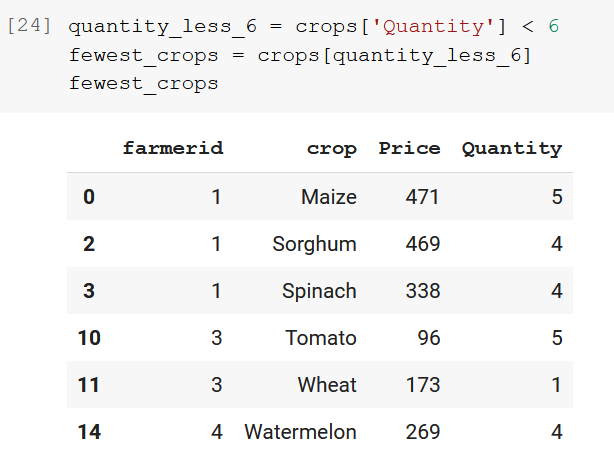
\includegraphics[width=0.6\linewidth]{img/fewest_crops.png}
	\end{figure}

\end{frame}

%%%%%%%%%%%%%%%%%%%%%%%%%%%%%%%%%%%%%%%%%%% Slide
\begin{frame}{Indexing and filtering}

	\textbf{Filtering}

	We can also use more than one condition at the same time:

	\begin{figure}
		\centering
		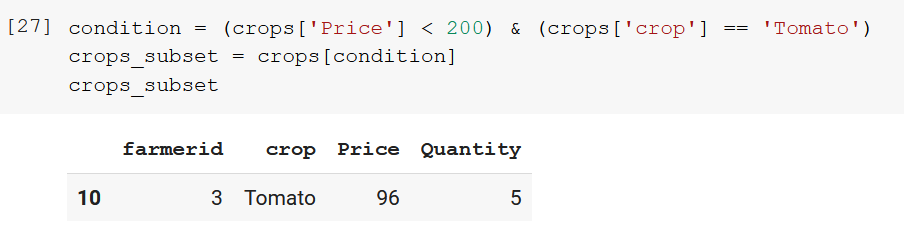
\includegraphics[width=0.9\linewidth]{img/crops_subset.png}
	\end{figure}

	\textbf{Important:} When using more than one condition, each of them must be enclosed in parentheses.

\end{frame}

%%%%%%%%%%%%%%%%%%%%%%%%%%%%%%%%%%%%%%%%%%% Section title slide
\sectionpic{Creating new columns}{img/section_slide}

%%%%%%%%%%%%%%%%%%%%%%%%%%%%%%%%%%%%%%%%%%% Slide
\begin{frame}{Creating new columns}

	\textbf{Creating new columns}

	\begin{itemize}
		\item To create a new column in a dataframe, we define it using the brackets as in:
	\end{itemize}
	
	\hspace{7mm} \texttt{df[new\_col\_name] = value}
	
	\begin{itemize}
		\item Other than a value, we can use columns operations to define new columns
	\end{itemize}

\end{frame}

%%%%%%%%%%%%%%%%%%%%%%%%%%%%%%%%%%%%%%%%%%% Slide
\begin{frame}{Creating new columns}

	\textbf{Creating new columns}

	\begin{figure}
		\centering
		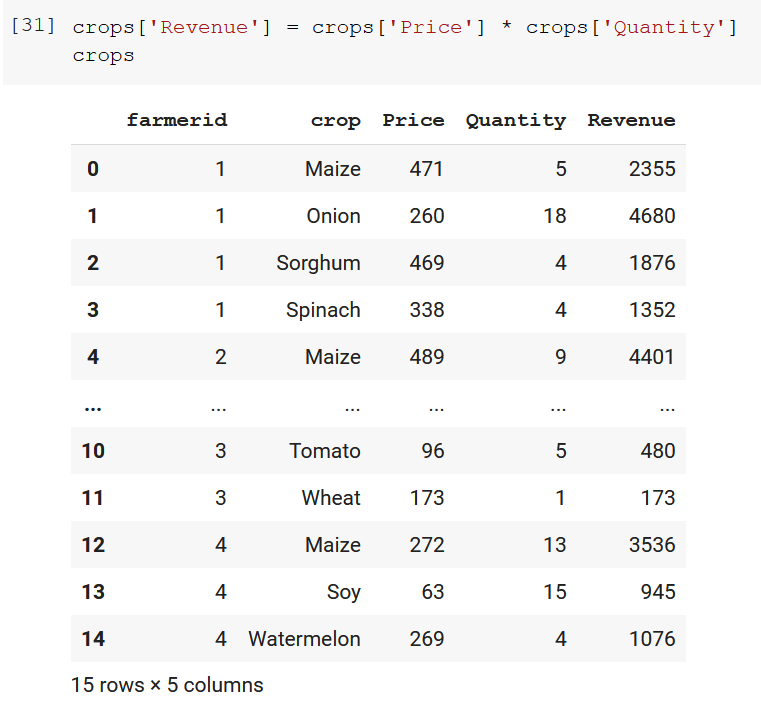
\includegraphics[width=0.5\linewidth]{img/column_generation.png}
	\end{figure}

\end{frame}

%%%%%%%%%%%%%%%%%%%%%%%%%%%%%%%%%%%%%%%%%%% Section title slide
\sectionpic{Group by}{img/section_slide}

%%%%%%%%%%%%%%%%%%%%%%%%%%%%%%%%%%%%%%%%%%% Slide
\begin{frame}{Group by}

	\textbf{Group by}

	\begin{itemize}
		\item The syntax to group a dataframe is:
	\end{itemize}

	\hspace{7mm} \texttt{df.groupby(by = col\_name).sum()}

	\begin{itemize}
		\item This will return a grouped dataframe by \texttt{col\_name}, where every other column contains a sum of its previous values by \texttt{col\_name}
		\item Other possible operations are: \texttt{.mean()}, \texttt{.std()}, and \texttt{.quantile()}
		\item We can also group by more than one column, by replacing \texttt{col\_name} with a list of strings containing the column names to group by
	\end{itemize}

\end{frame}

%%%%%%%%%%%%%%%%%%%%%%%%%%%%%%%%%%%%%%%%%%% Slide
\begin{frame}{Group by}

	\textbf{Group by}

	\begin{figure}
		\centering
		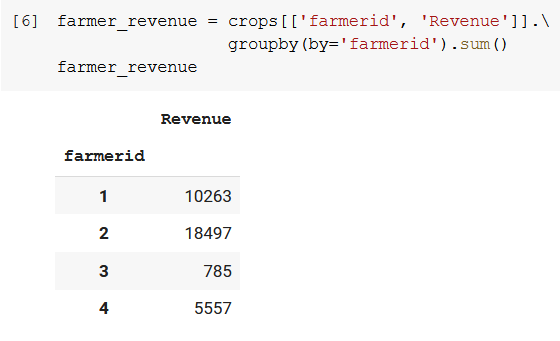
\includegraphics[width=\linewidth]{img/groupby.png}
	\end{figure}

\end{frame}

%%%%%%%%%%%%%%%%%%%%%%%%%%%%%%%%%%%%%%%%%%% Slide
\begin{frame}{Group by}

	\textbf{Group by}

	\begin{multicols}{2}
		\begin{itemize}
			\item After grouping, the resulting dataframe has the group column as index
			\item This means that \texttt{farmer\_revenue} has a \textbf{meaningful index} now, an index that has information itself and is different than the row number
			\item Meaningful indices can be useful in some cases, but that's out of the topics we'll cover today
		\end{itemize}
		\begin{figure}
			\centering
			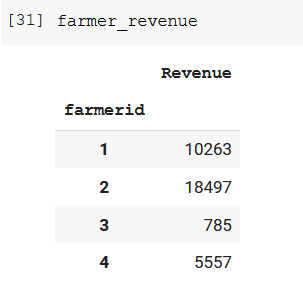
\includegraphics[width=0.8\linewidth]{img/farmer_revenue.png}
		\end{figure}
	\end{multicols}{2}

\end{frame}

%%%%%%%%%%%%%%%%%%%%%%%%%%%%%%%%%%%%%%%%%%% Slide
\begin{frame}{Group by}

	\textbf{Group by}

	To move \texttt{farmerid} back to the columns, use the attribute \texttt{.reset\_index()}. We could have also used the argument \texttt{as\_index=False} in \texttt{.groupby()} in the first place for this.

	\begin{multicols}{2}
		\begin{figure}
			\centering
			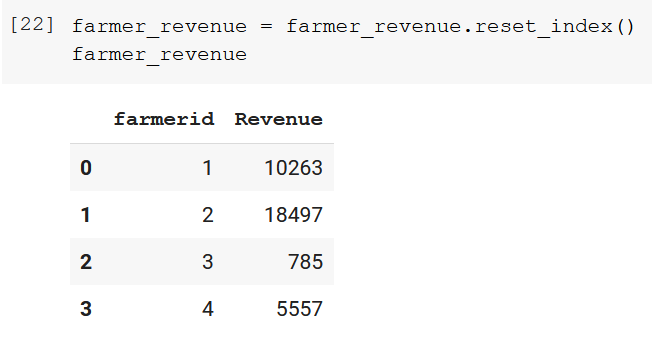
\includegraphics[width=0.8\linewidth]{img/reset_index.png}
		\end{figure}
		\begin{figure}
			\centering
			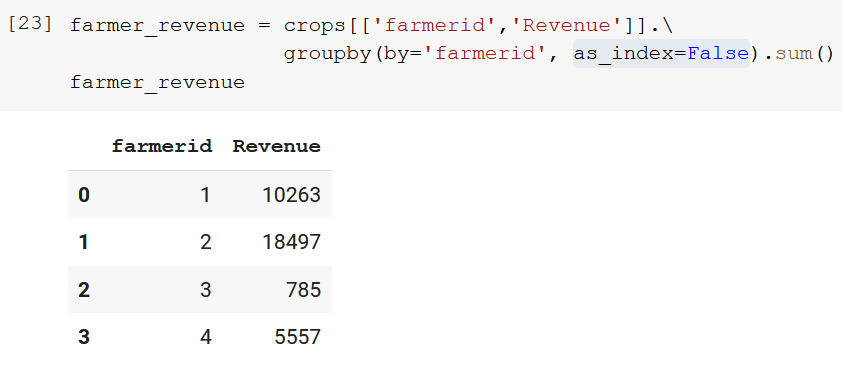
\includegraphics[width=\linewidth]{img/groupby_no_index.png}
		\end{figure}
	\end{multicols}{2}

\end{frame}

%%%%%%%%%%%%%%%%%%%%%%%%%%%%%%%%%%%%%%%%%%% Section title slide
\sectionpic{Merge and append}{img/section_slide}

%%%%%%%%%%%%%%%%%%%%%%%%%%%%%%%%%%%%%%%%%%% Slide
\begin{frame}{Merge and append}

	\textbf{Merge}

	The basic syntax to merge two dataframes is:

	\hspace{7mm} \texttt{pd.merge(left=left\_df,}
	\newline \hspace*{25.5mm} \texttt{right=right\_df,}
	\newline \hspace*{25.5mm} \texttt{left\_on=col\_name,}
	\newline \hspace*{25.5mm} \texttt{right\_on=col\_name,}
	\newline \hspace*{25.5mm} \texttt{how=merge\_type)}

\end{frame}

%%%%%%%%%%%%%%%%%%%%%%%%%%%%%%%%%%%%%%%%%%% Slide
\begin{frame}{Merge and append}

	\textbf{Merge}

	The type of merge can be one of these values:

	\begin{itemize}
		\item \textbf{"left":} keep only observations from left df, similar to Stata's \texttt{keep master} option
		\item \textbf{"right":} keep only observations from right df, similar to Stata's \texttt{keep using}
		\item \textbf{"inner":} keep all matched observations, similar to \texttt{keep match}
		\item \textbf{"outer":} keep all observations, similar to not using Stata's \texttt{keep} option
	\end{itemize}

\end{frame}

%%%%%%%%%%%%%%%%%%%%%%%%%%%%%%%%%%%%%%%%%%% Slide
\begin{frame}{Merge and append}

	\textbf{Merge}

	To show how a merge is done, we first read an second dataframe:

	\begin{figure}
		\centering
		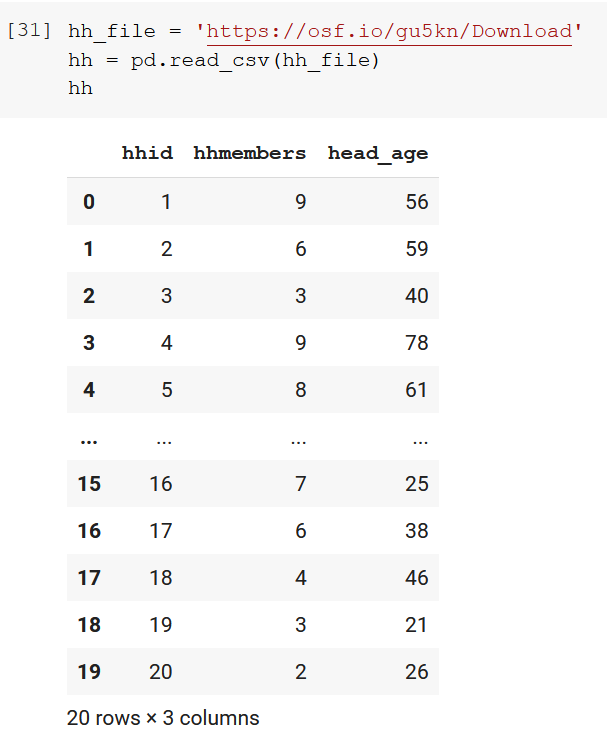
\includegraphics[width=0.33\linewidth]{img/hh_df.png}
	\end{figure}

\end{frame}

%%%%%%%%%%%%%%%%%%%%%%%%%%%%%%%%%%%%%%%%%%% Slide
\begin{frame}{Merge and append}

	\textbf{Merge}

	\begin{multicols}{2}

		\begin{figure}
			\centering
			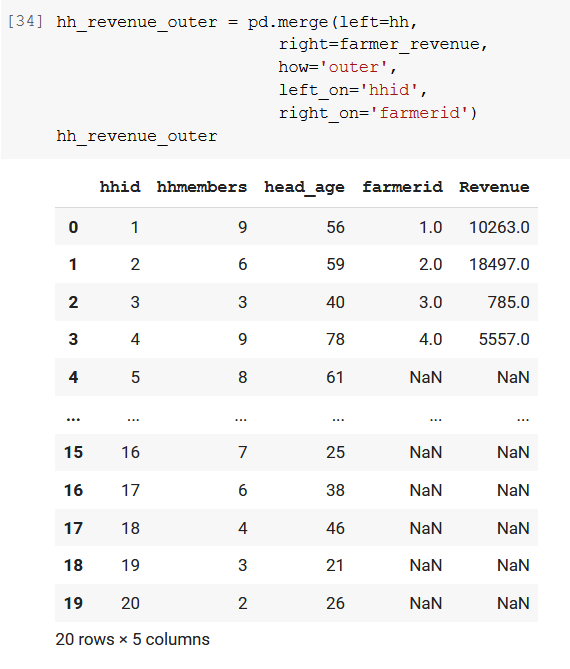
\includegraphics[width=0.85\linewidth]{img/outer_merge.png}
		\end{figure}
		\begin{figure}
			\centering
			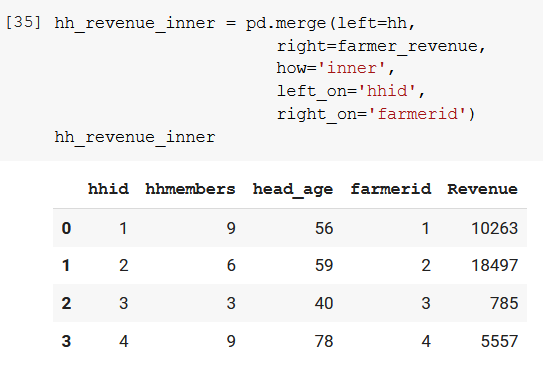
\includegraphics[width=0.85\linewidth]{img/inner_merge.png}
		\end{figure}

	\end{multicols}{2}

\end{frame}

%%%%%%%%%%%%%%%%%%%%%%%%%%%%%%%%%%%%%%%%%%% Slide
\begin{frame}{Merge and append}

	\textbf{Merge}

	\begin{itemize}
		\item An inner merge will only keep the matched observations
		\item An outer merge will include all obervations
		\item In Pandas we don't specify if it's a merge from one to many or one to one
	\end{itemize}

\end{frame}

%%%%%%%%%%%%%%%%%%%%%%%%%%%%%%%%%%%%%%%%%%% Slide
\begin{frame}{Merge and append}

	\textbf{Merge}

	\begin{itemize}
		\item If a column is repeated in both dataframes, they will be added with the suffixes "\texttt{\_x}" and "\texttt{\_y}" to differentiate them. To avoid this, it's better to index only the columns we'll need to use before merging
		\item If we want to generate a column with the source of each row, we need to add the argument \texttt{indicator=True}. This is similar to the variable \texttt{\_merge} that Stata creates by default
	\end{itemize}

\end{frame}

%%%%%%%%%%%%%%%%%%%%%%%%%%%%%%%%%%%%%%%%%%% Slide
\begin{frame}{Merge and append}

	\textbf{Append}

	Appending two dataframes in Pandas:

	\hspace{7mm} \texttt{df.append(other\_df)}

	This appends \texttt{other\_df} to the end of \texttt{df}.

\end{frame}

%%%%%%%%%%%%%%%%%%%%%%%%%%%%%%%%%%%%%%%%%%% Slide
\begin{frame}{Merge and append}

	\textbf{Append}

	\begin{multicols}{2}

		\begin{figure}
			\centering
			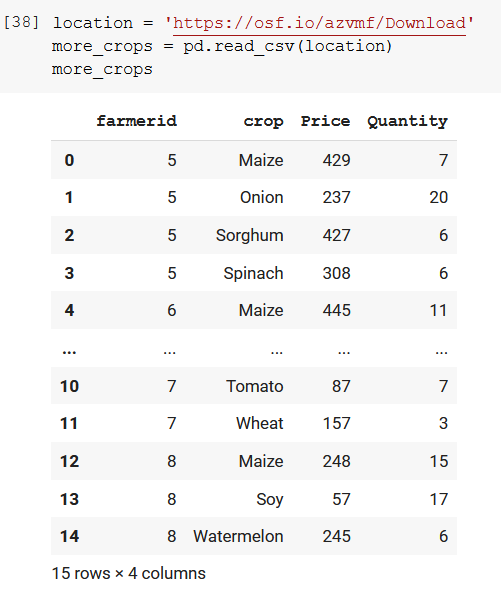
\includegraphics[width=0.8\linewidth]{img/more_crops.png}
		\end{figure}
		\begin{figure}
			\centering
			\includegraphics[width=0.9\linewidth]{img/crops_total.png}
		\end{figure}

	\end{multicols}{2}

\end{frame}

%%%%%%%%%%%%%%%%%%%%%%%%%%%%%%%%%%%%%%%%%%% Slide
\begin{frame}{Merge and append}

	\textbf{Append}

	\begin{itemize}
		\item The resulting dataframe has 30 rows but the last value we see in the index is 14
		\item This is because append operations keep the index of the original dataframes intact
		\item To reset the index, we can use the attribute \texttt{.reset\_index(drop=True)} or the argument \texttt{ignore\_index=True} inside \texttt{.append()}
	\end{itemize}

\end{frame}

%%%%%%%%%%%%%%%%%%%%%%%%%%%%%%%%%%%%%%%%%%% Slide
\begin{frame}{Merge and append}

	\textbf{Append}

	\begin{multicols}{2}

		\begin{figure}
			\centering
			\includegraphics[width=0.87\linewidth]{img/crops_total_reset_index.png}
		\end{figure}
		\begin{figure}
			\centering
			\includegraphics[width=\linewidth]{img/crops_total_ignore_index.png}
		\end{figure}

	\end{multicols}{2}

\end{frame}

%%%%%%%%%%%%%%%%%%%%%%%%%%%%%%%%%%%%%%%%%%% Section title slide
\sectionpic{Replacing column values}{img/section_slide}

%%%%%%%%%%%%%%%%%%%%%%%%%%%%%%%%%%%%%%%%%%% Slide
\begin{frame}{Replacing column values}

	\textbf{Replacing column values}

	\begin{itemize}
		\item To replace an entire column with a single value, we just overwrite the column with: \texttt{df[col\_name] = new\_value}
		\item To replace certain values based on a condition, we use \texttt{df.loc[]} again
	\end{itemize}

\end{frame}

%%%%%%%%%%%%%%%%%%%%%%%%%%%%%%%%%%%%%%%%%%% Slide
\begin{frame}{Replacing column values}

	\textbf{Replacing column values}

	The syntax to replace values based on conditions is:

	\texttt{df.loc[row\_indexer, col\_indexer] = new\_value}

	\begin{itemize}
		\item \textbf{row\_indexer:} a list or Pandas series with booleans. Dataframe observations with a value of \texttt{True} for their corresponding row order will be replaced
		\item \textbf{col\_indexer:} a string with the column name to replace. Can be a list of strings for more than column
		\item \textbf{new\_value:} the new value we want to use
	\end{itemize}

\end{frame}

%%%%%%%%%%%%%%%%%%%%%%%%%%%%%%%%%%%%%%%%%%% Slide
\begin{frame}{Replacing column values}

	\textbf{Replacing column values}

	\begin{figure}
		\centering
		\includegraphics[width=0.57\linewidth]{img/replace_values.png}
	\end{figure}

\end{frame}

%%%%%%%%%%%%%%%%%%%%%%%%%%%%%%%%%%%%%%%%%%% Section title slide
\sectionpic{Descriptive statistics}{img/section_slide}

%%%%%%%%%%%%%%%%%%%%%%%%%%%%%%%%%%%%%%%%%%% Slide
\begin{frame}{Descriptive statistics}

	\textbf{Descriptive statistics}

	\begin{multicols}{2}

		\begin{itemize}
			\item The attribute \texttt{.describe()} returns a dataframe with descriptive statistics
			\item By default, it includes only columns with numeric types
			\item It can also be applied on a single column when indexing
		\end{itemize}

		\begin{figure}
			\centering
			\includegraphics[width=0.85\linewidth]{img/crops_total_describe.png}
		\end{figure}

	\end{multicols}{2}


\end{frame}

%%%%%%%%%%%%%%%%%%%%%%%%%%%%%%%%%%%%%%%%%%% Slide
\begin{frame}{Descriptive statistics}

	\textbf{Descriptive statistics}

	\begin{multicols}{2}

		\begin{itemize}
			\item We can also get statistics for individual columns
			\item Some attributes for this are: \texttt{.mean()}, \texttt{.sum()}, \texttt{.std()}, \texttt{.min()}, \texttt{.max()}, \texttt{.median()}, \texttt{.quantile()}, \texttt{.count()}
		\end{itemize}

		\begin{figure}
			\centering
			\includegraphics[width=\linewidth]{img/desc_stats.png}
		\end{figure}

	\end{multicols}{2}

\end{frame}

%%%%%%%%%%%%%%%%%%%%%%%%%%%%%%%%%%%%%%%%%%% Slide
\begin{frame}{Descriptive statistics}

	\textbf{Descriptive statistics}

	To tabulate the values of a column, use the atribute \texttt{.value\_counts()}

	\begin{figure}
		\centering
		\includegraphics[width=0.5\linewidth]{img/value_counts.png}
	\end{figure}

	You can use the argument \texttt{dropna=False} to include the counts of \texttt{NaN} values

\end{frame}

%%%%%%%%%%%%%%%%%%%%%%%%%%%%%%%%%%%%%%%%%%% Section title slide
\sectionpic{Exporting to csv}{img/section_slide}

%%%%%%%%%%%%%%%%%%%%%%%%%%%%%%%%%%%%%%%%%%% Slide
\begin{frame}{Exporting to csv}

	\textbf{Exporting to csv}

	Finally, we can export the dataframe \texttt{crops\_total} to a csv file using the attribute \texttt{.to\_csv()}

	\begin{figure}
		\centering
		\includegraphics[width=0.6\linewidth]{img/to_csv.png}
	\end{figure}

	Pandas by default includes a column with the index when exporting. We use the argument \texttt{index=False} to omit it.

\end{frame}

%%%%%%%%%%%%%%%%%%%%%%%%%%%%%%%%%%%%%%%%%%% Slide
\begin{frame}{Data processing}

	\textbf{Downloading from Colab}

	\begin{itemize}
		\item Given that we used Colab for these exercises, the resulting file was exported to Colab's cloud storage
		\item To download the file to yor computer, click the folder icon to the left, locate the file, click on the vertical ellipsis next to it and click \texttt{Download}
	\end{itemize}

	\begin{figure}
		\centering
		\includegraphics[width=0.45\linewidth]{img/download_colab.png}
	\end{figure}

\end{frame}


\end{document}
